\documentclass[10pt,a4paper]{article}
\usepackage[margin=1.5cm,top=1.3cm,bottom=1.2cm]{geometry}
\usepackage{amsmath,amssymb}
\usepackage{graphicx,float,booktabs,enumitem,microtype}
\usepackage[font=footnotesize,labelfont=bf,skip=3pt,belowskip=0pt,aboveskip=3pt]{caption}
\usepackage{titlesec}
\usepackage{xcolor}
\usepackage[hidelinks]{hyperref}

% AUTO-GENERATED by simulation/mvm/tables.py -- do not edit
\newcommand{\Bcomp}{50\,000}
\newcommand{\Bmain}{100\,000}
\newcommand{\areLapHundred}{1.74}
\newcommand{\areLapThousand}{1.91}
\newcommand{\areNormalSim}{0.638}
\newcommand{\areNormalThy}{0.637}
\newcommand{\areTfiveSim}{0.960}
\newcommand{\areTfiveThy}{0.961}
\newcommand{\areTfourSim}{1.127}
\newcommand{\areTfourThy}{1.125}
\newcommand{\areTthreeSim}{1.598}
\newcommand{\areTthreeThy}{1.621}
\newcommand{\areTukeyFive}{0.83}
\newcommand{\areTukeyTen}{1.00}
\newcommand{\areTukeyTwenty}{1.24}
\newcommand{\bdKHL}{30}
\newcommand{\bdKHuber}{51}
\newcommand{\bdKMean}{1}
\newcommand{\bdKMedian}{51}
\newcommand{\bdKTrim}{11}
\newcommand{\bdPctHL}{29.7}
\newcommand{\bdPctHuber}{50.5}
\newcommand{\bdPctMean}{1.0}
\newcommand{\bdPctMedian}{50.5}
\newcommand{\bdPctTrim}{10.9}
\newcommand{\biasShiftFiveMean}{0.50}
\newcommand{\biasShiftFiveMedian}{0.07}
\newcommand{\biasShiftTenMean}{1.00}
\newcommand{\biasShiftTenMedian}{0.14}
\newcommand{\cauchyEffMed}{0.81}
\newcommand{\cauchyEffThy}{0.81}
\newcommand{\cauchyMeanNvarTen}{1.7\times10^{6}}
\newcommand{\cauchyMeanNvarThousand}{1.1\times10^{9}}
\newcommand{\cauchyMeanQfiftyRange}{0.997--1.003}
\newcommand{\cauchyMedNvarThousand}{2.45}
\newcommand{\cauchyMedNvarThy}{2.47}
\newcommand{\cauchyMedQfiftyTen}{0.33}
\newcommand{\cauchyMedQfiftyThousand}{0.033}
\newcommand{\cauchyQFiftyThy}{1.0}
\newcommand{\cauchyQNinetyNineThy}{64}
\newcommand{\cauchyQNinetyThy}{6.3}
\newcommand{\cmpCauchyHL}{3.44}
\newcommand{\cmpCauchyHuber}{3.63}
\newcommand{\cmpCauchyMedian}{2.50}
\newcommand{\cmpCauchyTrim}{5.22}
\newcommand{\cmpLaplaceHL}{1.37}
\newcommand{\cmpLaplaceHuber}{1.46}
\newcommand{\cmpLaplaceMean}{2.01}
\newcommand{\cmpLaplaceMedian}{1.17}
\newcommand{\cmpLaplaceTrim}{1.52}
\newcommand{\cmpNormalHL}{1.06}
\newcommand{\cmpNormalHuber}{1.07}
\newcommand{\cmpNormalMean}{1.01}
\newcommand{\cmpNormalMedian}{1.56}
\newcommand{\cmpNormalTrim}{1.07}
\newcommand{\cmpShiftFiveHL}{2.28}
\newcommand{\cmpShiftFiveHuber}{2.11}
\newcommand{\cmpShiftFiveMean}{30.93}
\newcommand{\cmpShiftFiveMedian}{2.16}
\newcommand{\cmpShiftFiveTrim}{2.24}
\newcommand{\cmpShiftOneHL}{1.12}
\newcommand{\cmpShiftOneHuber}{1.11}
\newcommand{\cmpShiftOneMean}{2.96}
\newcommand{\cmpShiftOneMedian}{1.58}
\newcommand{\cmpShiftOneTrim}{1.11}
\newcommand{\cmpShiftTenHL}{6.41}
\newcommand{\cmpShiftTenHuber}{5.68}
\newcommand{\cmpShiftTenMean}{109.84}
\newcommand{\cmpShiftTenMedian}{3.94}
\newcommand{\cmpShiftTenTrim}{15.86}
\newcommand{\cmpTfiveHL}{1.33}
\newcommand{\cmpTfiveHuber}{1.33}
\newcommand{\cmpTfiveMean}{1.65}
\newcommand{\cmpTfiveMedian}{1.70}
\newcommand{\cmpTfiveTrim}{1.33}
\newcommand{\cmpTthreeHL}{1.60}
\newcommand{\cmpTthreeHuber}{1.60}
\newcommand{\cmpTthreeMean}{2.97}
\newcommand{\cmpTthreeMedian}{1.84}
\newcommand{\cmpTthreeTrim}{1.63}
\newcommand{\cmpTukeyTenHL}{1.32}
\newcommand{\cmpTukeyTenHuber}{1.31}
\newcommand{\cmpTukeyTenMean}{1.81}
\newcommand{\cmpTukeyTenMedian}{1.79}
\newcommand{\cmpTukeyTenTrim}{1.31}
\newcommand{\icMedian}{1.25}
\newcommand{\maxRelSE}{0.6}
\newcommand{\mseShiftFiveMean}{0.31}
\newcommand{\mseShiftFiveMedian}{0.022}
\newcommand{\mseShiftTenMean}{1.10}
\newcommand{\mseShiftTenMedian}{0.039}
\newcommand{\nvarMeanNormalThousand}{0.99}
\newcommand{\nvarMedNormalTen}{1.38}
\newcommand{\nvarMedNormalThousand}{1.56}
\newcommand{\nvarMedNormalTwentyFive}{1.55}
\newcommand{\ratioShiftFive}{14}
\newcommand{\ratioShiftTen}{28}
\newcommand{\scHL}{1.60}
\newcommand{\scHuber}{1.67}
\newcommand{\scMedian}{1.27}
\newcommand{\scTrim}{1.63}
\newcommand{\seedValue}{20261110}
\newcommand{\tCross}{4.68}
                                  % auto-generated numbers (simulation/mvm/tables.py)
\graphicspath{{../simulation/results/figures/}}

\definecolor{accent}{HTML}{184f95}
\definecolor{ink2}{HTML}{52514e}
\titleformat{\section}{\normalsize\bfseries\color{accent}}{\thesection}{0.5em}{}
\titlespacing*{\section}{0pt}{5pt}{2pt}
\setlength{\parindent}{0pt}\setlength{\parskip}{2.5pt}
\setlist{nosep,leftmargin=1.1em,itemsep=1pt}
\pagestyle{empty}
\renewcommand{\arraystretch}{0.96}
\newcommand{\Var}{\operatorname{Var}}
\newcommand{\ARE}{\operatorname{ARE}}
\newcommand{\CRLB}{\mathrm{CRLB}}
\newcommand{\repourl}{github.com/ParthSarda5/mean-vs-median}   % <- edit if the repository is named differently

\begin{document}
\fontsize{9.5}{11.3}\selectfont

{\raggedright
{\Large\bfseries\color{accent} Simulation Study: Sample Mean vs.\ Sample Median}\\[1pt]
{\small\color{ink2} MT3194 Statistical Inference \;|\; Group 11 (Bhumika, Parth, Satyam, Sriharipriya, Vishwabharathi) \;|\; simulation component\par}}
\vspace{1pt}{\color{accent}\hrule height 0.6pt}\vspace{1pt}

\section{Design}
\textbf{Estimators.} Sample mean $\bar X_n$ and median $M_n$, plus three middle-ground estimators: the 10\% trimmed mean, the Huber M-estimator ($k=1.345$, MAD scale; 95\% efficient at the normal) and Hodges--Lehmann (median of Walsh averages; ARE $3/\pi$ at the normal).
\textbf{Models} (i.i.d., centred at $\theta=0$): $N(0,1)$; Student $t_\nu$, $\nu\in\{1,2,3,4,5,10,30\}$ ($t_1$ is the Cauchy); Laplace; Tukey scale contamination $(1-\varepsilon)N(0,1)+\varepsilon N(0,3^2)$; asymmetric outliers $(1-\varepsilon)N(0,1)+\varepsilon N(10,1)$, $\varepsilon\in\{.01,.05,.10,.20\}$. $\bar X_n$ and $M_n$ run at $n\in\{10,25,50,100,500,1000\}$ with $B=\Bmain$ replications; the comparators at $n\in\{25,100\}$ with $B=\Bcomp$. Under the outlier model both estimators are biased for $\theta=0$, so we compare MSE.
\textbf{Metrics.} Bias, variance and MSE, with Monte Carlo standard errors from 20 independent batches (relative s.e.\ of every variance in Table~\ref{tab:are}: at most \maxRelSE\%); $n\Var$ against first-order theory ($n\Var(\bar X_n)=\sigma^2$, $n\Var(M_n)\to[4f(m)^2]^{-1}$, Cram\'er--Rao bound $[nI(\theta)]^{-1}$); and $\ARE=\Var(\bar X_n)/\Var(M_n)$ against $4\sigma^2f(m)^2$, where values above 1 favour the median. With infinite variance we report quantiles of $|\text{error}|$ and running estimates instead.
\textbf{Reproducibility.} Master seed \seedValue, an independent random stream per cell; code, data and 35 tests are in the repository (\texttt{\repourl}); every number below is generated from the saved results.

\begin{figure}[H]
\centering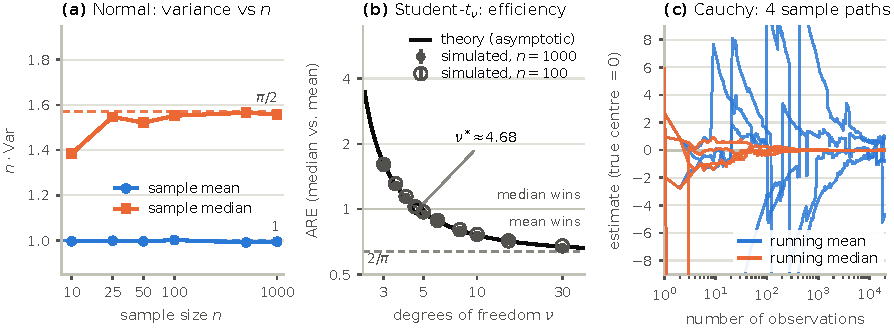
\includegraphics[width=\textwidth]{fig_core.pdf}
\caption{(a) $n\Var$ at $N(0,1)$ (95\% Monte Carlo bars); dashed: limits $1$ and $\pi/2$. (b) Simulated $\Var(\bar X)/\Var(M)$ for $t_\nu$ against the asymptotic curve; the median wins left of $\nu^*$. (c) Running mean and median on four Cauchy streams.}
\label{fig:core}
\end{figure}

\begin{table}[H]
\centering\footnotesize\setlength{\tabcolsep}{4.2pt}
\caption{Efficiency of the mean and the median ($B=\Bmain$). Bold: median more efficient. $^{\ddagger}$CRLB$/(n\Var)$ at $n=1000$; entries marginally above 1 are Monte Carlo noise. ``--'': $\Var(\bar X_n)=\infty$, so the simulated ratio is meaningless.}
\label{tab:are}
\begin{tabular}{@{}lrrrrrrrr@{}}
\toprule
 & \multicolumn{3}{c}{$n\cdot\mathrm{Var}$ at $n{=}1000$} & \multicolumn{3}{c}{ARE $=\mathrm{Var}(\bar X)/\mathrm{Var}(M)$} & \multicolumn{2}{c}{eff.\ vs CRLB$^{\ddagger}$}\\
\cmidrule(lr){2-4}\cmidrule(lr){5-7}\cmidrule(l){8-9}
Model & mean & median & med.\ thy & $n{=}100$ & $n{=}1000$ & theory & mean & median\\
\midrule
$N(0,1)$ & 0.99 & 1.56 & 1.57 & 0.645 & 0.638 & 0.637 & 1.01 & 0.64\\
$t_{10}$ & 1.24 & 1.64 & 1.65 & 0.761 & 0.758 & 0.757 & 0.95 & 0.72\\
$t_{5}$ & 1.66 & 1.73 & 1.73 & 0.975 & 0.960 & 0.961 & 0.80 & 0.77\\
$t_{4}$ & 2.01 & 1.78 & 1.78 & \textbf{1.140} & \textbf{1.127} & \textbf{1.125} & 0.70 & 0.78\\
$t_{3}$ & 2.97 & 1.86 & 1.85 & \textbf{1.603} & \textbf{1.598} & \textbf{1.621} & 0.50 & 0.81\\
$t_{2}$ & $\infty$ & 2.00 & 2.00 & -- & -- & \textbf{$\infty$} & 0.00 & 0.83\\
Cauchy ($t_1$) & $\infty$ & 2.45 & 2.47 & -- & -- & \textbf{$\infty$} & 0.00 & 0.81\\
Laplace & 2.00 & 1.05 & 1.00 & \textbf{1.735} & \textbf{1.909} & \textbf{2.000} & 0.50 & 0.96\\
Tukey $\varepsilon{=}0.10$ & 1.80 & 1.81 & 1.80 & 1.013 & 0.998 & 0.998 & 0.70 & 0.70\\
\bottomrule
\end{tabular}

\end{table}

\section{Results}
\textbf{Normal and $t$ models (Fig.~\ref{fig:core}a,b; Table~\ref{tab:are}).} At $N(0,1)$ the mean attains the bound ($n\Var=\nvarMeanNormalThousand$ at $n=1000$), while $n\Var(M_n)$ rises from \nvarMedNormalTen\ at $n=10$ (even $n$ averages two central order statistics) to $\nvarMedNormalThousand$ at $n=1000$, giving $\ARE=\areNormalSim$ against $2/\pi=\areNormalThy$: the median needs about 57\% more data. Across the $t$ family the simulated ARE reproduces $4\sigma^2f(0)^2$ to within Monte Carlo error (e.g.\ $t_3$: \areTthreeSim\ vs \areTthreeThy; $t_4$: \areTfourSim\ vs \areTfourThy). The median overtakes the mean at $\nu^*=\tCross$: $\ARE=\areTfourThy$ at $\nu=4$ but $\areTfiveThy$ at $\nu=5$. For Laplace data the median is the MLE and the ARE tends to 2, though slowly (\areLapHundred\ at $n=100$, \areLapThousand\ at $n=1000$), reflecting the cusp of the density at its median.

\textbf{Cauchy and infinite variance (Fig.~\ref{fig:core}c).} The sample mean of Cauchy data has the law of a single observation, so its $|\text{error}|$ quantiles (50/90/99\%) stay at \cauchyQFiftyThy/\cauchyQNinetyThy/\cauchyQNinetyNineThy\ for every $n$ (simulated medians: \cauchyMeanQfiftyRange) and $n\Var(\bar X_n)$ explodes (\ensuremath{\cauchyMeanNvarTen} at $n=10$, \ensuremath{\cauchyMeanNvarThousand} at $n=1000$). The median is consistent: its median $|\text{error}|$ falls from \cauchyMedQfiftyTen\ to \cauchyMedQfiftyThousand, and $n\Var(M_n)=\cauchyMedNvarThousand$ matches $\pi^2/4=\cauchyMedNvarThy$, i.e.\ efficiency \cauchyEffMed\ against the bound (theory $8/\pi^2=\cauchyEffThy$).

\textbf{Contamination (Fig.~\ref{fig:robust}d,e).} Symmetric scale contamination erodes the mean's advantage steadily: $\ARE=\areTukeyFive$ at $\varepsilon=.05$, $\areTukeyTen$ at $\varepsilon=.10$ and $\areTukeyTwenty$ at $\varepsilon=.20$, so a 10\% fraction of observations with three times the spread already makes the two estimators equally good. Asymmetric outliers are far worse for the mean: its bias is $10\varepsilon$ (\biasShiftFiveMean\ at $\varepsilon=.05$) against \biasShiftFiveMedian\ for the median, and its MSE is \mseShiftFiveMean\ versus \mseShiftFiveMedian\ (a factor \ratioShiftFive) at $\varepsilon=.05$ and a factor \ratioShiftTen\ at $\varepsilon=.10$; even $\varepsilon=.01$ triples the mean's $n\cdot$MSE (\cmpShiftOneMean\ vs.\ \cmpNormalMean\ when clean).
\textbf{Sensitivity and breakdown (Fig.~\ref{fig:robust}f,g).} $\mathrm{SC}_n$ is the finite-sample influence function: it grows linearly for the mean but is bounded for all others, at $\pm\scMedian$ for the median (theory $\pm1/(2\varphi(0))=\pm\icMedian$) and $\scTrim$--$\scHuber$ for the other three. In the breakdown experiment the mean fails at $k=\bdKMean$ ($\bdPctMean\%$), the trimmed mean at $k=\bdKTrim$ ($\bdPctTrim\%$), Hodges--Lehmann at $k=\bdKHL$ ($\bdPctHL\%$; theory $29.3\%$) and the median and Huber at $k=\bdKMedian$ ($\bdPctMedian\%$, the maximum possible).
\textbf{Middle-ground estimators (Table~\ref{tab:comp}).} At the normal the trimmed mean, Huber and HL give up only 6--7\% ($n\cdot$MSE $\cmpNormalHL$--$\cmpNormalHuber$ vs.\ $\cmpNormalMean$) whereas the median gives up 55\% ($\cmpNormalMedian$). For $t_5$, $t_3$ and Tukey contamination they beat \emph{both} the mean and the median (e.g.\ $t_5$: $\cmpTfiveHuber$ vs.\ $\cmpTfiveMean$/$\cmpTfiveMedian$). The median is best only when tails are very heavy or outliers numerous: Laplace ($\cmpLaplaceMedian$), Cauchy ($\cmpCauchyMedian$) and 10\% outliers ($\cmpShiftTenMedian$ vs.\ Huber $\cmpShiftTenHuber$, HL $\cmpShiftTenHL$).

\begin{figure}[H]
\centering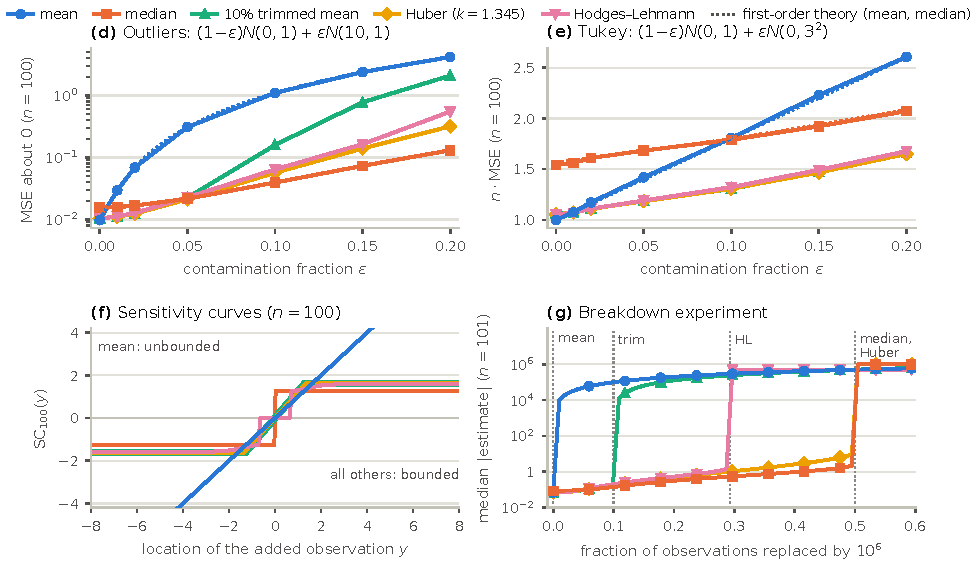
\includegraphics[width=\textwidth]{fig_robust.pdf}
\caption{Robustness ($n=100$ unless stated). (d,e) MSE vs.\ contamination; dotted: first-order theory (with bias terms $10\varepsilon$ and $m_\varepsilon$ in (d)). (f) $\mathrm{SC}_n(y)=n[T(x_1,\dots,x_{n-1},y)-T(x_1,\dots,x_{n-1})]$, $x_i=\Phi^{-1}\big(\tfrac{i-1/2}{n-1}\big)$. (g) $k$ of $n=101$ clean points replaced by $10^6$; vertical lines: theoretical breakdown points.}
\label{fig:robust}
\end{figure}

\begin{table}[H]
\centering\footnotesize\setlength{\tabcolsep}{5pt}
\caption{$n\cdot\mathrm{MSE}$ about $\theta=0$ at $n=100$ ($B=\Bcomp$; Monte Carlo error about 1\%). Lowest in bold (ties at printed precision share it). The mean has no finite MSE for Cauchy data.}
\label{tab:comp}
\begin{tabular}{@{}lrrrrr@{}}
\toprule
Model & mean & median & 10\% trim & Huber & HL\\
\midrule
\emph{$N(0,1)$, theory ($n\to\infty$)} & 1.00 & 1.57 & 1.06 & 1.05 & 1.05\\
\midrule
$N(0,1)$ & \textbf{1.01} & 1.56 & 1.07 & 1.07 & 1.06\\
$t_{5}$ & 1.65 & 1.70 & \textbf{1.33} & \textbf{1.33} & \textbf{1.33}\\
$t_{3}$ & 2.97 & 1.84 & 1.63 & \textbf{1.60} & \textbf{1.60}\\
Laplace & 2.01 & \textbf{1.17} & 1.52 & 1.46 & 1.37\\
Cauchy ($t_1$) & $\infty$ & \textbf{2.50} & 5.22 & 3.63 & 3.44\\
Tukey $\varepsilon{=}0.10$ & 1.81 & 1.79 & \textbf{1.31} & \textbf{1.31} & 1.32\\
Outliers $\varepsilon{=}0.10$ & 109.84 & \textbf{3.94} & 15.86 & 5.68 & 6.41\\
\bottomrule
\end{tabular}

\end{table}

\section{Practical guidelines}
\begin{itemize}
\item \textbf{Clean, near-normal data (light tails, no outliers):} use the mean; the median wastes about 36\% of the information ($\ARE\approx0.64$).
\item \textbf{Heavy tails ($t_\nu$ with $\nu\le4$, or infinite variance) or $\gtrsim10\%$ symmetric contamination:} prefer the median; with Cauchy-type data the mean does not converge at all.
\item \textbf{Asymmetric gross outliers:} never use the raw mean: 1\% contamination triples its $n\cdot$MSE, and at 5--10\% it is \ratioShiftFive--\ratioShiftTen\ times worse than the median; prefer the median or a robust compromise.
\item \textbf{When unsure:} Huber or Hodges--Lehmann cost under 7\% at the normal and are never far from the best, and beat both mean and median in the moderate-tail scenarios.
\item \textbf{Caveats.} Asymptotic ARE is accurate for $n\gtrsim100$ except for cusp-like densities (Laplace); under skewness the mean and median target different parameters, so comparisons presume symmetry.
\end{itemize}
{\footnotesize\color{ink2}\textbf{Refs.} Morris, White \& Crowther (2019), \emph{Stat.\ Med.} 38 (simulation-study design); Tukey (1960); Andrews et al.\ (1972) \emph{Robust Estimates of Location}; Hodges \& Lehmann (1963) \emph{Ann.\ Math.\ Stat.}; Huber \& Ronchetti (2009) \emph{Robust Statistics}; Hampel et al.\ (1986) \emph{Robust Statistics}.}

\end{document}
